\documentclass{report}

\input{~/dev/latex/template/preamble.tex}
\input{~/dev/latex/template/macros.tex}

\title{\Huge{}}
\author{\huge{Nathan Warner}}
\date{\huge{}}
\pagestyle{fancy}
\fancyhf{}
\lhead{Warner \thepage}
\rhead{}
% \lhead{\leftmark}
\cfoot{\thepage}
\setborder
% \usepackage[default]{sourcecodepro}
% \usepackage[T1]{fontenc}

\begin{document}
    % \maketitle
        \begin{titlepage}
       \begin{center}
           \vspace*{1cm}
    
           \textbf{Elementary Statistics Chapters 1-4 Exam Prep}
    
           \vspace{0.5cm}
           JJC Stat128
            
                
           \vspace{1.5cm}
            A Document By: \\ 
           \textbf{Nathan Warner}
    
           \vfill
                
                
           \vspace{0.8cm}
         
           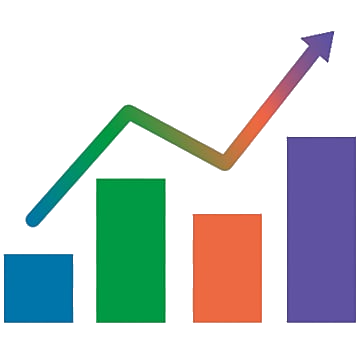
\includegraphics[width=0.4\textwidth]{./../lectures/1-4/figures/2.png} \\
           July 08,2023 \\
           Computer Science \\
           Northern Illinois University\\
           United States\\
           
                
       \end{center}
    \end{titlepage}
    \tableofcontents
    \pagebreak \bigbreak \noindent
    \section{Vocab}
    \begin{itemize}
        \item \textbf{Population:} The entire group to be studied is called the population.
        \item \textbf{Sample:} In statistics, it is often impractical or impossible to get access to the entire \textbf{population}, which is why we only look at a \textbf{sample.} A sample is a \textbf{subset} of the population being studied.
        \item \textbf{Individual:} An individual is a person or object that is a member of the population being studied.
        \item \textbf{Statistic:} A statistic is a numerical summary of a sample.
        \item \textbf{Descriptive Statistics:} Descriptive statistics consist of organizing and summarizing data. Descriptive statistics describe data through numerical summaries, tables, and graphs.
        \item \textbf{Inferential Statistics:} inferential Statistics uses methods that take a result from a sample, extend it to the population, and measure the reliability of the result.
        \item \textbf{Parameter:} A parameter is a numerical summary of a population.
        \item \textbf{Variables:} The characteristics of the individuals in a study. Variables vary, which means they can take on different values.
        \item \textbf{Constants:} Variables that do not vary. Inferential statistics is not necessary with constants.
        \item \textbf{Qualitative, or categorical variables} allow for the classification of individuals base on some attribute or characteristic.
        \item \textbf{Quantitative variables} provide numerical measures of individuals. The values of a quantitative variable can be added or subtracted and provide meaningful results.
        \item A \textbf{discrete variable} is a quantitative variable that has either a finite number of possible values or a countable number of possible values. A discrete variable cannot take on every possible value between any two possible values.
        \item A \textbf{continuous variable} is a quantitative variable that has an infinite number of possible values that are not countable. A continuous variable may take on every possible value between any two values. Continuous variables typically result from measurement. Continuous variables are often rounded. If a certain make of car gets 24 miles per gallon (mpg) of gasoline, its miles per gallon must be greater than or equal to 23.5 and less than 24.5, or $23.5 \leq mpg \leq 24.5$
        \item The list of observed values for a variable is \textbf{data.}
        \item \textbf{Qualitative data} are observations corresponding to a \textbf{qualitative variable.}
        \item \textbf{Quantitative data} are observations corresponding to a quantitative variable.
        \item \textbf{Discrete data} are observations corresponding to a discrete variable.
        \item \textbf{Continuous data} are observations corresponding to a continuous variable.
            \item \textbf{Explanatory Variable:} An explanatory variable, also known as an independent variable or predictor variable, is a variable that is manipulated or controlled by researchers in an experiment or study. It is the variable that is hypothesized to have an impact on the outcome or dependent variable. 
            \item \textbf{Lurking variable}: An explanatory variable that was not considered in a study, but that affects the value of the response variable.
            \item \textbf{Response Variable}: The response variable, also known as the dependent variable or outcome variable, is the variable that is measured or observed to determine the effect or response of the explanatory variable(s). It is the variable that researchers are interested in studying or predicting. 
            \item \textbf{Confounding:} Occurs when the effects of two or more explanatory variables are not separated. Therefore, any relation that may exist between an explanatory variable and the response variable may be due to some other variable or variables not accounted for in the study.
            \item \textbf{Census:} List of individuals in a population along with certain characteristics of each individual.
            \item \textbf{Random Sampling:} The process of using chance to select individuals from a population to be included in the sample.
            \item \textbf{Simple Random Sampling:} A sample of size $n$  from a population of size $N $  is obtained through simple random sampling if every possible sample of size $n$  has an equal chance of occurring. The sample is then called a simple random sample.
                \begin{itemize}
                    \item $n < N $
                \end{itemize}
            \item \textbf{frame:} a list of all the individuals within the population.
        \begin{itemize}
            \item \textbf{Stratified sample}: is obtained by dividing the population into nonoverlapping groups called strata and then obtaining a simple random sample from each stratum. The individuals within each stratum should be homogenous (similar) in some way.
                \begin{itemize}
                    \item Within Stratified samples, the number of individuals sampled from each stratum should be proportional to the size of the strata in the population.
                \end{itemize}
            \item \textbf{Systematic sample} is obtained by selecting every $k$th individual from the population. The first individual selected corresponds to a number between 1 and $k$
            \item \textbf{Cluster sample} is obtained by selecting all individuals within a randomly selected collection or group of individuals.
            \item \textbf{Convenience sample:} the individuals are easily obtained and not based on randomness.
        \end{itemize}
            \item \textbf{Bias:} If the results of the sample are not representative of the population. Sampling bias means that the technique used to obtain the sample's individuals tends to favor one part of the  population over another. Any convenience sample has sampling bias because the individuals are not chosen through a random sample.
            \item \textbf{Undercoverage:} Occurs when the proportion of one segment of the population is lower in a sample than it is in the population. This can result if the frame used to obtain the sample is incomplete or not representative of the population.
            \item \textbf{Sampling bias:} sampling bias is a bias in which a sample is collected in such a way that some members of the intended population have a lower or higher sampling probability than others. It results in a biased sample of a population in which all individuals, or instances, were not equally likely to have been selected
            \item \textbf{Nonresponse bias:} exists when individuals selected to be in the sample who do not respond to the survey have different opinions from those who do
                \begin{itemize}
                    \item This can be controlled with \textbf{callbacks}.
                    \item This can also be controlled with \textbf{rewards or incentives}
                \end{itemize}
            \item \textbf{Response bias:} Exists when the answers on a survey do not reflect the true feelings of the respondent.
            \item \textbf{Open Question:} Allows the respondent to choose his or her response
            \item \textbf{Closed Question:} requires the respondent to choose from a list of predetermined responses
            \item \textbf{Nonsampling errors:} result from undercoverage, nonresponse bias, response bias, or data-entry error. Such errors could also be present in a census.
            \item \textbf{Sampling error:} results from using a sample to estimate information about a population. This type of error occurs because a sample gives incomplete information about a population.
            \item \textbf{Experiment:} is a controlled study conducted to determine the effect of varying one or more explanatory variables or \textbf{factors} has on a response variable. 
            \item \textbf{Factor:} A variable whose effect on the response variable is to be assessed by the experimenter
            \item \textbf{Treatment:} Any combination of the values of the factors is called a treatment
            \item \textbf{Experimental Unit (or subject)} is a person, object or some other well-defined item upon which a treatment is applied
            \item \textbf{Control Group:} Serves as a baseline treatment that can be used to compare to other treatments.
            \item \textbf{Placebo:} is an innocuous medication, such as a sugar tablet, that looks, tastes, and smells like the experimental medication.
            \item \textbf{Blinding:} refers to nondisclosure of the treatment an experimental unit is receiving.
            \item \textbf{Single-blind} experiment is one in which the experimental unit (or subject) does not know which treatment he or she is receiving.
            \item \textbf{Double-blind} experiment is one in which neither the experimental unit nor the researcher in contact with the experimental unit knows which treatment the experimental unit is receiving.
            \item \textbf{Design:} To design an experiment means to describe the overall plan in conducting the experiment. Conducting an experiment requires a series of steps.
            \item \textbf{completely randomized design:} is one in which each experimental unit is randomly assigned to a treatment.
            \item \textbf{matched-pairs design:} is an experimental design in which the experimental units are paired up. The pairs are selected so that they are related in some way (that is, the same person before and after a treatment, twins, husband and wife, same geographical location, and so on). There are only two levels of treatment in a matched-pairs design.
            \item \textbf{A frequency distribution} lists each category of data and the number of occurrences for each category of data.
            \item \textbf{The relative frequency} is the proportion (or percent) of observations within a category and is found using the formula
                \begin{align*}
                    Relative\ frequency = \frac{Frequency}{Sum\ of\ all\ frequency}
                .\end{align*}
            \item \textbf{A relative frequency distribution} lists each category of data together with the relative frequency.
            \item \textbf{A bar graph} is constructed by labeling each category of data on either the horizontal or vertical axis and the frequency or relative frequency of the category on the other axis. Rectangles of equal width are drawn for each category. The height of each rectangle represents the category's frequency or relative frequency.
            \item \textbf{A Pareto chart} is a bar graph whose bars are drawn in decreasing order of frequency or relative frequency.
            \item \textbf{A pie chart} is a circle divided into sectors. Each sector represents a category of data. The area of each sector is proportional to the frequency of the category.
            \item A \textbf{histogram} is constructed by drawing rectangles for each class of data. The height of each rectangle is the frequency or relative frequency of the class. The width of each rectangle is the same, and the rectangles touch each other.
            \item \textbf{Classes: } The Categories in which data is grouped
            \item \textbf{lower class limit:} the smallest value within the class 
            \item \textbf{upper class limit:} the largest value within the class 
            \item \textbf{Class Width: }  is the difference between consecutive lower class limits.
            \item A table is \textbf{open ended} if the first class has no lower class limit or the last class has no upper class limit
            \item We draw a \textbf{dot plot} by placing each observation horizontally in increasing order and placing a dot above the observation each time it is observed.
            \item \textbf{uniform distribution:} frequency of each value of the variable is evenly spread across the values of the variable. 
            \item \textbf{bell-shaped distribution:} highest frequency occurs in the middle and frequencies tail off to the left and right of the middle.
            \item \textbf{skewed right:} the tail to the right of the peak is longer than the tail to the left of the peak
            \item \textbf{skewed left:} tail to the left of the peak is longer than the tail to the right of the peak.
            \item \textbf{The arithmetic mean} of a variable is computed by adding all the values of the variable in the data set and dividing by the number of observations.
            \item \textbf{The population arithmetic mean}, $\mu$, (pronounced "mew"), is a parameter that is computed using data from all the individuals in a population.
                \begin{align*}
                    \mu = \frac{x_{1}+x_{2} + x_{N}}{N} = \frac{\summation{}{}x_{i}}{N}
                .\end{align*}
            \item \textbf{The sample arithmetic mean}, $\bar{x}$ (pronounced x-bar"), is a statistic that is computed using data from individuals in a sample.
                \begin{align*}
                    \bar{x} = \frac{x_{1}+x_{2} + x_{n}}{n} = \frac{\summation{}{}x_{i}}{n}
                .\end{align*}
            \item \textbf{The median} of a variable is the value that lies in the middle of the data when arranged in ascending order. We use $M$  to represent the median.
                \begin{itemize}
                    \item For odd $n$:
                        \begin{align*}
                            M = \frac{n+1}{2}
                        .\end{align*}
                    \item For even $n$:
                        \begin{align*}
                            M = Average\ of\ \frac{n}{2}, \frac{n}{2}+1
                        .\end{align*}
                \end{itemize}
            \item A numerical summary of data is said to be \textbf{resistant} if observations that are extreme (very large or small) relative to the data do not affect its value substantially.
                \begin{itemize}
                    \item So the median is resistant, but the mean is not resistant.
                \end{itemize}
            \item \textbf{The mode} of a variable is the observation of the variable that occurs most frequently in the data set.
                \begin{itemize}
                    \item If no observation occurs more than once, we say that the data have \textbf{no mode}.
                \end{itemize}
            \item \textbf{Bimodal:} If the data has two modes
            \item \textbf{Multimodal:} If the data has more than two modes
            \item A numerical summary of data is said to be \textbf{resistant} if observations that are extreme (very large or small) relative to the data do not affect its value substantially.
                \begin{itemize}
                    \item So the median is resistant, but the mean is not resistant.
                \end{itemize}
            \item \textbf{Dispersion:} Degree to which the data are spread out. 
            \item \textbf{Range:} The range, $r $, of a variable is the difference between the largest and smallest data value. That is,
                \begin{align*}
                    range = R = Largest\ data\ value- smallest\ data\ value
                .\end{align*}
                \textbf{Note:} Range is \textbf{not} resistant
            \item \textbf{Deviation:} a deviation refers to the difference between an individual data point and a central value, such as the mean or median. It represents how much a particular data point varies or deviates from the average or typical value in a data set. When can comopute a deviation with:
                \begin{align*}
                    Individual\ data\ point - mean
                .\end{align*}
                We call this calculation, "deviation about the mean"
                \bigbreak \noindent 
                \textbf{Note:} The sum of the deviations about the mean always equals zero
            \item \textbf{The population standard deviation} of a variable is the square root of the sum of squared deviations about the population mean divided by the number of observations in the population, $N$. The population standard deviation is symbolically represented by $\sigma$ (lowercase Greek sigma). The formula is given by:
                \begin{align*}
                    \sigma = \sqrt{\frac{(x_{1} - \mu)^{2} + (x_{2}-\mu)^{2}+...+(x_{N}-\mu)^{2}}{N}} \\
                    = \sqrt{\frac{\summation{}{}(x_{i}-\mu)^{2} }{N}}
                .\end{align*}
                \textbf{Note:} Standard Deviation is \textbf{not} resistant
            \item \textbf{The sample standard deviation}, $s $, of a variable is the square root of the sum of squared deviations about the sample mean divided by $n-1 $, where $n$  is the sample size. The formula is given as
                \begin{align*}
                    s = \sqrt{\frac{(x_{1} - \overline{x})^{2}+(x_{2}-\overline{x})^{2}+...+(x_{n}-\overline{x})^{2}}{n-1}}\\
                    = \sqrt{\frac{\summation{}{}(x_{i}-\overline{x})^{2}}{n-1}}
                .\end{align*}
                \textbf{Note:} Standard Deviation is \textbf{not} resistant
            \item  we call $n-1$ the \textbf{degrees of freedom} because the first $n-1 $  observations have freedom to be any value, but the $n^{th}$ observation has no freedom. It must be whatever value forces the sum of the deviations about the mean to equal zero.
            \item The variance of a variable is the square of the standard deviation.
                \begin{itemize}
                    \item  \textbf{The population variance} is \textbf{$\sigma^{2}$} 
                    \item \textbf{The Sample Variance} is $s^{2}$
                \end{itemize}
                \textbf{Note:} The units of measure in variance are squared values. So if the variable is measured in dollars, the variance is measured in dollars squared. This makes interpreting the variance difficult.
             \item \textbf{Class Midpoint:} The class midpoint is the sum of consecutive lower class limits divided by 2
             \item \textbf{Approximate Population Mean (if we do not have access to the original data, ie data has been grouped (classed) and frequency chart has already been made)}
                \begin{align*}
                    \mu =\frac{\sum x_i f_i}{\sum f_i} \\
                     =\frac{x_1 f_1+x_2 f_2+\cdots+x_n f_n}{f_1+f_2+\cdots+f_n}
                .\end{align*}
            where: $\quad x_i$ is the midpoint or value of the $i$ th class  \\
            $f_i$ is the frequency of the $i$ th class  \\
            $n$ is the number of classes
            \item \textbf{Approximate Sample Mean (if we do not have access to the original data, ie data has been grouped (classed) and frequency chart has already been made)}
                \begin{align*}
                    \overline{x} = \frac{\sum x_{i}f_{i}}{\sum f_{i}} \\
                     = \frac{x_{1}f_{1} + x_{2} f_{2} + ... +x_{n} f_{n}}{f_{1} + f_{2} + ... + f_{n}}
                .\end{align*}
            where: $\quad x_i$ is the midpoint or value of the $i$ th class  \\
            $f_i$ is the frequency of the $i$ th class  \\
            $n$ is the number of classes
            \item \textbf{The weighted mean}, $\overline{x}_{w}$, of a variable is found by multiplying each value of the variable by its corresponding weight, adding these products, and dividing this sum by the sum of the weights. It can be expressed using the formula
                \begin{align*}
                    \overline{x}_{w} = \frac{\sum w_{i}x_{i}}{w_{i}} = \frac{w_{1} + x_{1} + w_{2} + x_{2} + ... + w_{n} + x_{n}}{w_{1} + w_{2} + ... + w_{n}}
                .\end{align*}
                Where: \quad $w_{i}$ is the weight of the $i^{th}$ observation \\
                $x_{i}$ is the value of the $i^{th}$ observation.
            \item \textbf{Approximate Population Standard Deviation (if we do not have access to the original data, ie data has been grouped (classed) and frequency chart has already been made)}
                \begin{align*}
                    \sigma = \sqrt{\frac{\sum(x_{i} - \mu)^{2}f_{i}}{\sum f_{i}}}
                .\end{align*}
                Where: \quad  $x_{i}$ is the midpoint or value of the ith class \\
                $f_{i}$ is the frequency of the $i^{th}$ class
            \item \textbf{Approximate Sample Standard Deviation (if we do not have access to the original data, ie data has been grouped (classed) and frequency chart has already been made)}
                \begin{align*}
                    s = \sqrt{\frac{\sum(x_{i}-\overline{x})^{2}f_{i}}{\sum f_{i} -1}}
                .\end{align*}
                Where: \quad  $x_{i}$ is the midpoint or value of the ith class \\
                $f_{i}$ is the frequency of the $i^{th}$ class
             \item \textbf{The z-score} represents the distance that a data value is from the mean in terms of the number of standard deviations. We find it by subtracting the mean from the data value and dividing this result by the standard deviation.
                 \begin{itemize}
                     \item \textbf{Population Z-score}
                 \end{itemize}
                 \begin{align*}
                      z = \frac{x - \mu}{\sigma}
                 .\end{align*}
                 \begin{itemize}
                     \item \textbf{Sample Z-score}
                 \end{itemize}
                 \begin{align*}
                     z =\frac{x-\overline{x}}{s}
                 .\end{align*}
                 \textbf{Note:} The Z-score is unitless. It has mean  0 and a standard deviation of 1 \\
                 \textbf{Round z-scores to the nearest hundredth}
             \item  The median is a special case of a general concept called the \textbf{percentile.}
             \item \textbf{the $k^{th}$  percentile,} denoted $P_{k} $,  of a set of data is a value such that $k $  percent of the observations are less than or equal to the value.
                \item The most common percentiles are \textbf{quartiles}, which divide data sets into fourths, or four equal parts.
                \item The \textbf{interquartile range, IQR,} is the range of the middle $50\% $  of the observations in a data set. That is, the IQR is the difference between the first and third quartiles and is found using this formula  
                    \begin{align*}
                        IQR = Q_{3} - Q_{1}
                    .\end{align*}
                \item \textbf{Outliers:} When analyzing data, we must check for extreme observations, called outliers. Outliers can occur by chance, because of errors in the measurement of a variable, during data entry, or from errors in sampling.
                \item \textbf{Fences} serve as cutoff points for determining outliers.
                    \begin{align*}
                        Lower\ Fence\ = Q_{1} - 1.5\cdot IQR \\
                        Upper\ Fence\ = Q_{3} + 1.5\cdot IQR
                    .\end{align*}
        \item The \textbf{five-number summary} of a set of data consists of the smallest data value, $Q_{1} $  the median, $Q_{3} $  and the largest data value. We use the five-number summary to learn information about the extremes of the data set. The summary is organized as follows:
        \begin{center}
           Minimum $Q_{1} $ $M$ $Q_{3} $  Maximum
        \end{center}
        \item \textbf{bivariate data:} data in which two variables are measured on an individual. For example, we might want to know whether the amount of cola consumed per week is related to a person's bone density. The individuals would be the people in the study, and the two variables would be the amount of cola consumed weekly and bone density.
        \item \textbf{The response (dependent) variable} is the variable whose value can be explained by the value of the explanatory (or predictor or independent) variable.
        \item \textbf{A scatter diagram} is a graph that shows the relationship between two quantitative variables measured on the same individual. Each individual in the data set is represented by a point in the scatter diagram. The explanatory variable is plotted on the horizontal axis, and the response variable is plotted on the vertical axis.
        \item Two variables that are linearly related are \textbf{positively associated} when above-average values of one variable are associated with above-average values of the other variable (or below-average values of one variable are associated with below-average values of the other variable). That is, two variables are positively associated if, whenever the value of one variable increases, the value of the other variable also increases.
        \item Two variables that are linearly related are \textbf{negatively associated} when above-average values of one variable are associated with below-average values of the other variable. That is, two variables are negatively associated if, whenever the value of one variable increases, the value of the other variable decreases.
        \item The \textbf{linear correlation coefficient}, or Pearson product moment correlation coefficient, is a measure of the strength and direction of the linear relation between two quantitative variables. The Greek letter $\rho $ (rho) represents the population correlation coefficient, and $r $ represents the sample correlation coefficient. We present only the formula for the sample correlation coefficient.
            \begin{align*}
                r =\frac{\sum\left(\frac{x_i-\bar{x}}{s_x}\right)\left(\frac{y_i-\bar{y}}{s_y}\right)}{n-1}
            .\end{align*}
            Where:
            \bigbreak \noindent 
                $x_i$ is the $i$ th observation of the explanatory variable \\
                $\overline{x}$ is the sample mean of the explanatory variable \\
                $s_{x} $is the sample standard deviation of the explanatory variable \\
                $y_i$ is the $i$ th observation of the response variable \\
                $\overline{y}$ is the sample mean of the response variable \\
                $\mathbf{S}_y$ is the sample standard deviation of the response variable \\
                $n$ is the number of individuals in the sample

        \item \textbf{The least-squares regression line} minimizes the sum of the squared errors (or residuals). This line minimizes the sum of the squared vertical distance between the observed values of $y$  and those predicted by the line, $\hat{y}$  (read “y-hat"). We represent this as $\sum residuals^{2}$
            \begin{align*}
               \hat{y} = b_{1}x + b_{0} 
            .\end{align*}
            Where:
            \begin{align*}
                b_{1} = r \cdot \frac{s_{y}}{s_{x}}\ \text{is the slope of the least-squares regression line}
            .\end{align*}
            And:
            \begin{align*}
                b_{0} = \overline{y} -b_{1}\overline{x}\ \text{is the y-Intercept of the least-squares regression line} 
            .\end{align*}
        \item The observed distance for this club-head speed is 274 yards. The difference between the observed and predicted values of y is the error, or \textbf{residual}.
            \begin{align*}
                Residual\ = observed - predicted
            .\end{align*}
        \item \textbf{The coefficient of determination}, $R^{2}$, measures the proportion of total variation in the response variable that is explained by the least-squares regression line.
            \begin{align*}
                R^{2} = r^{2}
            .\end{align*}
        \item \textbf{An influential observation} significantly affects the least-squares regression line's slope and/or y-intercept. (It also affects the value of the correlation coefficient.) Methods exist for determining whether a particular observation is influential; however, they are beyond the scope of this course. Nonetheless, we can still get a sense as to whether a particular observation is influential right now.
        \item the difference in our predicted value, and our actual value, is due to factors (variables) other than the club-head speed (wind speed and position of the ball on the club face, for example) and to random error. The differences just discussed are called \textbf{deviations}.
        \item \textbf{Total Deviation:} The deviation between the observed value, y, and mean value, $\overline{y} $, of the response variable.
            \begin{align*}
                &y - \overline{y} \\
                &Or: \text{Explained Deviation + Unexplained Deviation}
            .\end{align*}
        \item \textbf{Explained Deviation:} The deviation between the predicted value, $\hat{y} $, and mean value, $\overline{y} $, of the response variable.
            \begin{align*}
                \hat{y}-\overline{y}
            .\end{align*}
        \item \textbf{Unexplained Deviation:} The deviation between the observed value, y, and predicted value, $\hat{y} $, of the response variable
            \begin{align*}
                y - \hat{y}
            .\end{align*}
        \item     If a plot of the residuals against the explanatory variable shows the spread of the residuals increasing or decreasing as the explanatory variable increases, then a strict requirement of the linear model is violated.     This requirement is called \textbf{constant error variance}. The statistical term for constant error variance is \textbf{homoscedasticity}

        \item \textbf{A marginal distribution} of a variable is a frequency or relative frequency distribution of either the row or column variable in the contingency table.
        \item \textbf{A conditional distribution} lists the relative frequency of each category of the response variable, given a specific value of the explanatory variable in the contingency table.
        \item \textbf{Simpson's Paradox}, which describes a situation in which an association between two variables inverts or goes away when a third variable is introduced to the analysis.
        \end{itemize}

        \pagebreak \bigbreak \noindent
        \section{Formulas}
        \bigbreak \noindent 
        \begin{itemize}
                        \item \textbf{The relative frequency} is the proportion (or percent) of observations within a category and is found using the formula
                \begin{align*}
                    Relative\ frequency = \frac{Frequency}{Sum\ of\ all\ frequency}
                .\end{align*}

                    \item \textbf{The population arithmetic mean}, $\mu$, (pronounced "mew"), is a parameter that is computed using data from all the individuals in a population.
                \begin{align*}
                    \mu = \frac{x_{1}+x_{2} + x_{N}}{N} = \frac{\summation{}{}x_{i}}{N}
                .\end{align*}
            \item \textbf{The sample arithmetic mean}, $\bar{x}$ (pronounced x-bar"), is a statistic that is computed using data from individuals in a sample.
                \begin{align*}
                    \bar{x} = \frac{x_{1}+x_{2} + x_{n}}{n} = \frac{\summation{}{}x_{i}}{n}
                .\end{align*}
            \item \textbf{The median} of a variable is the value that lies in the middle of the data when arranged in ascending order. We use $M$  to represent the median.
                \begin{itemize}
                    \item For odd $n$:
                        \begin{align*}
                            M = \frac{n+1}{2}
                        .\end{align*}
                    \item For even $n$:
                        \begin{align*}
                            M = Average\ of\ \frac{n}{2}, \frac{n}{2}+1
                        .\end{align*}
                \end{itemize}
            \item \textbf{Range:} The range, $r $, of a variable is the difference between the largest and smallest data value. That is,
                \begin{align*}
                    range = R = Largest\ data\ value- smallest\ data\ value
                .\end{align*}
            \item \textbf{Deviation:} a deviation refers to the difference between an individual data point and a central value, such as the mean or median. It represents how much a particular data point varies or deviates from the average or typical value in a data set. When can comopute a deviation with:
                \begin{align*}
                    Individual\ data\ point - mean
                .\end{align*}


            \item \textbf{The population standard deviation} of a variable is the square root of the sum of squared deviations about the population mean divided by the number of observations in the population, $N$. The population standard deviation is symbolically represented by $\sigma$ (lowercase Greek sigma). The formula is given by:
                \begin{align*}
                    \sigma = \sqrt{\frac{(x_{1} - \mu)^{2} + (x_{2}-\mu)^{2}+...+(x_{N}-\mu)^{2}}{N}} \\
                    = \sqrt{\frac{\summation{}{}(x_{i}-\mu)^{2} }{N}}
                .\end{align*}
                \textbf{Note:} Standard Deviation is \textbf{not} resistant
            \item \textbf{The sample standard deviation}, $s $, of a variable is the square root of the sum of squared deviations about the sample mean divided by $n-1 $, where $n$  is the sample size. The formula is given as
                \begin{align*}
                    s = \sqrt{\frac{(x_{1} - \overline{x})^{2}+(x_{2}-\overline{x})^{2}+...+(x_{n}-\overline{x})^{2}}{n-1}}\\
                    = \sqrt{\frac{\summation{}{}(x_{i}-\overline{x})^{2}}{n-1}}
                .\end{align*}
                \textbf{Note:} Standard Deviation is \textbf{not} resistant
             \item \textbf{Approximate Population Mean (if we do not have access to the original data, ie data has been grouped (classed) and frequency chart has already been made)}
                \begin{align*}
                    \mu =\frac{\sum x_i f_i}{\sum f_i} \\
                     =\frac{x_1 f_1+x_2 f_2+\cdots+x_n f_n}{f_1+f_2+\cdots+f_n}
                .\end{align*}
            where: $\quad x_i$ is the midpoint or value of the $i$ th class  \\
            $f_i$ is the frequency of the $i$ th class  \\
            $n$ is the number of classes
            \item \textbf{Approximate Sample Mean (if we do not have access to the original data, ie data has been grouped (classed) and frequency chart has already been made)}
                \begin{align*}
                    \overline{x} = \frac{\sum x_{i}f_{i}}{\sum f_{i}} \\
                     = \frac{x_{1}f_{1} + x_{2} f_{2} + ... +x_{n} f_{n}}{f_{1} + f_{2} + ... + f_{n}}
                .\end{align*}
            where: $\quad x_i$ is the midpoint or value of the $i$ th class  \\
            $f_i$ is the frequency of the $i$ th class  \\
            $n$ is the number of classes
            \item \textbf{The weighted mean}, $\overline{x}_{w}$, of a variable is found by multiplying each value of the variable by its corresponding weight, adding these products, and dividing this sum by the sum of the weights. It can be expressed using the formula
                \begin{align*}
                    \overline{x}_{w} = \frac{\sum w_{i}x_{i}}{w_{i}} = \frac{w_{1} + x_{1} + w_{2} + x_{2} + ... + w_{n} + x_{n}}{w_{1} + w_{2} + ... + w_{n}}
                .\end{align*}
                Where: \quad $w_{i}$ is the weight of the $i^{th}$ observation \\
                $x_{i}$ is the value of the $i^{th}$ observation.
            \item \textbf{Approximate Population Standard Deviation (if we do not have access to the original data, ie data has been grouped (classed) and frequency chart has already been made)}
                \begin{align*}
                    \sigma = \sqrt{\frac{\sum(x_{i} - \mu)^{2}f_{i}}{\sum f_{i}}}
                .\end{align*}
                Where: \quad  $x_{i}$ is the midpoint or value of the ith class \\
                $f_{i}$ is the frequency of the $i^{th}$ class
            \item \textbf{Approximate Sample Standard Deviation (if we do not have access to the original data, ie data has been grouped (classed) and frequency chart has already been made)}
                \begin{align*}
                    s = \sqrt{\frac{\sum(x_{i}-\overline{x})^{2}f_{i}}{\sum f_{i} -1}}
                .\end{align*}
                Where: \quad  $x_{i}$ is the midpoint or value of the ith class \\
                $f_{i}$ is the frequency of the $i^{th}$ class
             \item \textbf{The z-score} represents the distance that a data value is from the mean in terms of the number of standard deviations. We find it by subtracting the mean from the data value and dividing this result by the standard deviation.
                 \begin{itemize}
                     \item \textbf{Population Z-score}
                 \end{itemize}
                 \begin{align*}
                      z = \frac{x - \mu}{\sigma}
                 .\end{align*}
                 \begin{itemize}
                     \item \textbf{Sample Z-score}
                 \end{itemize}
                 \begin{align*}
                     z =\frac{x-\overline{x}}{s}
                 .\end{align*}
                 \textbf{Note:} The Z-score is unitless. It has mean  0 and a standard deviation of 1 \\
                 \textbf{Round z-scores to the nearest hundredth}
                \item The \textbf{interquartile range, IQR,} is the range of the middle $50\% $  of the observations in a data set. That is, the IQR is the difference between the first and third quartiles and is found using this formula  
                    \begin{align*}
                        IQR = Q_{3} - Q_{1}
                    .\end{align*}
                \item \textbf{Fences} serve as cutoff points for determining outliers.
                    \begin{align*}
                        Lower\ Fence\ = Q_{1} - 1.5\cdot IQR \\
                        Upper\ Fence\ = Q_{3} + 1.5\cdot IQR
                    .\end{align*}

        \item The \textbf{five-number summary} of a set of data consists of the smallest data value, $Q_{1} $  the median, $Q_{3} $  and the largest data value. We use the five-number summary to learn information about the extremes of the data set. The summary is organized as follows:
        \begin{center}
           Minimum $Q_{1} $ $M$ $Q_{3} $  Maximum
        \end{center}
        \item The \textbf{linear correlation coefficient}, or Pearson product moment correlation coefficient, is a measure of the strength and direction of the linear relation between two quantitative variables. The Greek letter $\rho $ (rho) represents the population correlation coefficient, and $r $ represents the sample correlation coefficient. We present only the formula for the sample correlation coefficient.
            \begin{align*}
                r =\frac{\sum\left(\frac{x_i-\bar{x}}{s_x}\right)\left(\frac{y_i-\bar{y}}{s_y}\right)}{n-1}
            .\end{align*}
            Where:
            \bigbreak \noindent 
                $x_i$ is the $i$ th observation of the explanatory variable \\
                $\overline{x}$ is the sample mean of the explanatory variable \\
                $s_{x} $is the sample standard deviation of the explanatory variable \\
                $y_i$ is the $i$ th observation of the response variable \\
                $\overline{y}$ is the sample mean of the response variable \\
                $\mathbf{S}_y$ is the sample standard deviation of the response variable \\
                $n$ is the number of individuals in the sample

        \item \textbf{The least-squares regression line} minimizes the sum of the squared errors (or residuals). This line minimizes the sum of the squared vertical distance between the observed values of $y$  and those predicted by the line, $\hat{y}$  (read “y-hat"). We represent this as $\sum residuals^{2}$
            \begin{align*}
               \hat{y} = b_{1}x + b_{0} 
            .\end{align*}
            Where:
            \begin{align*}
                b_{1} = r \cdot \frac{s_{y}}{s_{x}}\ \text{is the slope of the least-squares regression line}
            .\end{align*}
            And:
            \begin{align*}
                b_{0} = \overline{y} -b_{1}\overline{x}\ \text{is the y-Intercept of the least-squares regression line} 
            .\end{align*}
        \item The observed distance for this club-head speed is 274 yards. The difference between the observed and predicted values of y is the error, or \textbf{residual}.
            \begin{align*}
                Residual\ = observed - predicted
            .\end{align*}
        \item \textbf{The coefficient of determination}, $R^{2}$, measures the proportion of total variation in the response variable that is explained by the least-squares regression line.
            \begin{align*}
                R^{2} = r^{2}
            .\end{align*}

        \item \textbf{Total Deviation:} The deviation between the observed value, y, and mean value, $\overline{y} $, of the response variable.
            \begin{align*}
                &y - \overline{y} \\
                &Or: \text{Explained Deviation + Unexplained Deviation}
            .\end{align*}
        \item \textbf{Explained Deviation:} The deviation between the predicted value, $\hat{y} $, and mean value, $\overline{y} $, of the response variable.
            \begin{align*}
                \hat{y}-\overline{y}
            .\end{align*}
        \item \textbf{Unexplained Deviation:} The deviation between the observed value, y, and predicted value, $\hat{y} $, of the response variable
            \begin{align*}
                y - \hat{y}
            .\end{align*}
        \item     If a plot of the residuals against the explanatory variable shows the spread of the residuals increasing or decreasing as the explanatory variable increases, then a strict requirement of the linear model is violated.     This requirement is called \textbf{constant error variance}. The statistical term for constant error variance is \textbf{homoscedasticity}


        \end{itemize}

        \pagebreak \bigbreak \noindent
        \section{Concepts To Know:}
        \begin{itemize}
    \item Statistics and Statistical Thinking.
    \begin{itemize}
        \item Describe Variability
        \item Understand Sources of variability
        \item The process of statistics
        \begin{enumerate}
            \item Identify the problem to be solved. It is important to clearly lay out the questions that the researcher wants answered, along with clearly specifying which population the study applies.
            \item Collect the data.
            \item Describe the data.
            \item Perform inference.
        \end{enumerate}
    \end{itemize}
    \item Inferential/Descriptive Statistics
    \begin{itemize}
        \item Inferential Statistics uses methods that take a result from a sample, extend it to the population, and measure the reliability of the result.
        \item Descriptive statistics consist of organizing and summarizing data. Descriptive statistics describe data through numerical summaries, tables, and graphs.
    \end{itemize}
    \item Variables
    \begin{itemize}
        \item Qualitative (Categorical) / Quantitative
        \item Discrete (count) / Continuous (measure)
    \end{itemize}
    \item Data
    \begin{itemize}
        \item Qualitative (Categorical) / Quantitative
        \item Discrete (count) / Continuous (measure)
    \end{itemize}
    \item Distinguish between an Observational Study and a Designed Experiment
    \item Explain the Various Types of Observational Studies
    \begin{itemize}
        \item Cross-sectional Studies: Observational studies that collect information about individuals at a specific point in time, or over a very short period of time.
        \item Case-control Studies: These studies are retrospective, meaning that they require individuals to look back in time or require the researcher to look at existing records. In case-control studies, individuals that have certain characteristics are matched with those that do not.
        \begin{itemize}
            \item Positive: Control group allows for a comparison
            \item Negative: Individuals must remember details
            \item Negative: Records might not exist
        \end{itemize}
        \item Cohort Studies: A cohort study first identifies a group of individuals to participate in the study (cohort). The cohort is then observed over a period of time. Over this time period, characteristics about the individuals are recorded. Because the data is collected over time, cohort studies are prospective.
        \begin{itemize}
            \item Advantage: Researcher does not need to rely on the memory of study participants or existing records.
            \item Disadvantage: Requires a lot of time.
            \item Disadvantage: Could be expensive.
        \end{itemize}
    \end{itemize}
    \item Effective Sampling Techniques:
    \begin{enumerate}
        \item Simple random sampling
        \item Stratified sampling
        \item Systematic sampling
        \item Cluster sampling
    \end{enumerate}
    \item Obtaining a Simple Random Sample Using Stat-Crunch or calculator
    \item Bonus:
    \begin{itemize}
        \item $nCk$ formula
        \item Probability formula
    \end{itemize}
    \item Obtain a Stratified Sample
    \item Obtain a Systematic Sample
    \begin{itemize}
        \item Choosing a value of $k$ if $N$ is not known
        \item Mathematically deducing a value of $k$ if $N$ is known
        \item Steps to deduce $k$ and compute sequence:
        \begin{enumerate}
            \item If possible, approximate the population size $N$.
            \item Determine the sample size desired, $n$.
            \item Divide $N$ by $n$ and round down to the nearest integer. This value is $k$.
            \item Randomly select a number between 1 and $k$, call this number $a$ (starting point).
            \item The sample will consist of the following individuals:
        \end{enumerate}
    \end{itemize}
    \item Obtain a Cluster Sample
    \begin{itemize}
        \item We conclude that if the clusters have homogeneous individuals, it is better to have more clusters with fewer individuals in each cluster.
        \item When each cluster is heterogeneous, fewer clusters with more individuals in each cluster are appropriate.
    \end{itemize}
    \item 3 sources of bias
    \item Steps in designing an experiment
    \item Explain a matched-pairs design
    \item Make Frequency Distribution Chart
    \item Make Relative Frequency Distribution Chart
    \item Make bar graph
    \item Dual bar graph
    \item Pie chart
    \item Creating Tables with classes (using bin function $\rightarrow$ data > bin)
    \item Histogram
    \item Determining the lower limit of the first class and class width formula
    \item Drawing a dot plot
    \item Identify Shape of a Distribution
    \item Most common graphical misrepresentations of data:
    \begin{itemize}
        \item Scale
        \item Inconsistent Scale
        \item Misplaced Origin
    \end{itemize}
    \item Finding population mean (formula)
    \item Finding a simple random sample from a population
    \item Finding sample mean (formula)
    \item Steps in finding median, finding median if $n$ is even and if $n$ is odd (formula)
    \item How to find mode
    \item When to use mean, median, or mode.
    \item Relation among the Mean, Median, and Distribution Shape
    \item Finding Range (formula)
    \item What is deviation about the mean? What should the sum of all these values be?
    \item Population Standard Deviation (formula)
    \begin{itemize}
        \item The sum of the deviations about the mean always equals zero
    \end{itemize}
    \item Sample Standard Deviation (formula)
    \item What does a higher standard deviation mean?
    \item Is the standard deviation resistant?
    \item What is variance?
    \item The empirical rule
    \item Approximate population mean (formula)
    \item Approximate sample mean (formula)
    \item Weighted mean (formula)
    \item Approximate population standard deviation (formula)
    \item Approximate sample standard deviation (formula)
    \item What is a z-score?
    \item Population z-score (formula)
    \item Sample z-score (formula)
    \item A z-score is unitless (mean=0, std.dev=1)
    \item Negative z-score
    \item Interpret percentiles
    \item Find and interpret quartiles
    \begin{itemize}
        \item Quartiles are resistant
    \end{itemize}
    \item Find IQR (formula)
    \item Deciding Which Measure of Central Tendency and Dispersion to Report
    \item Fences (finding fences) (formula)
    \item How fences find Outliers
    \item Five Number Summary
    \item Boxplots (Create them)
    \item Scatter plot axes
    \item Positive and negative association
    \item sample linear correlation (formula) 
    \item Properties of linear correlation cofficient
    \item Chart
    \item correlation causation
    \item equation of least-squares regression line (formula)
    \item use it to make predictions
    \item what is a residual (formula)
    \item sum of least squares residual
    \item Coefficient of determination 
    \item Three tyes of deviation and how to calculate (total deviation = explained vs unexplained)
    \item Finding the Coefficient of Determination
    \item is a linear model appropriate?
    \item is the variance of the residuals constant? 
    \item are their any outliers? 
    \item Marginal Distribution
    \item Conditional Distribution
    \item Simpson's Paradox
    \item Drawing bar graph of conditional distribution




    \end{itemize}
    
\end{document}
